\chapter{Game and AI Implementation}

The primary objective of this study is to design and develop a framework for the implementation and evaluation of artificial intelligence (AI) agents in Durak. Since framework in this game is tailored to support the application and evaluation of AI algorithms within the game environment, the focus of this chapter is to provide a high-level overview of the framework's architecture, including its capabilities for supporting the development and evaluation of AI agents for Durak.

%%%A more in-depth analysis of the implementation and functionality of the game model can be found in section \ref{devdoc} of the developer documentation, as well as in the user documentation provided in section \ref{userdoc}. These sections provide comprehensive information on the design and implementation of the game model, as well as its capabilities and usage for both developers and end users.

\section{OS support}

The game framework for Durak was tested on both Windows 10 and Linux operating systems to confirm compatibility and functionality. While this list is not exhaustive, and the framework may potentially run on other operating systems, these are the only ones that were formally tested. It is possible that the framework will operate correctly on other platforms, but this has not been verified.

\section{A High-Level View of the Framework}

The Durak AI framework includes a game model, AI agents, and a Command-Line Interface (CLI) that are implemented using the C\# programming language and targeted for the .NET Core 6 platform. C\# was selected as the programming language for the implementation of aforementioned projects in Durak due to its suitability for writing back-end systems. The language offers a range of reliable libraries and benefits from a highly optimized Just-In-Time (JIT) compiler, resulting in enhanced speed. These attributes made C\# an ideal choice for this development.

In order to run and test the program, the project has to be cloned from the repository and opened with an Integrated Development Environment (IDE) of user's choice. From the root directory of the project, the user can utilize the command line to enter the command 
\begin{lstlisting}[frame=single]
dotnet run --project CLI
\end{lstlisting}
, which will launch the Command-Line Interface (CLI) and provide guidance on how to proceed with experimentation. The CLI will provide further instructions on how to use and test the program (for additional information, please refer to Section \ref{CLI}.).

\subsection{Project Structure}
The game Durak is organized within a solution file, with the file extension ``.sln'', which is a type of file used to manage projects in Visual Studio. This solution includes three individual projects: 

\begin{itemize}

\item Model - A C\# library project contains the game logic for Durak.

\item Agent - A C\# library contains all of the implemented AI agents.

\item CLI - A C\# Command-Line Interface (CLI) project includes parameters for modifying the game model and agents settings in order to perform experiments.

The aforementioned components will be further discussed in the following subsections.

\end{itemize}

\subsection{Game Model}

The game model, which represents the current state of the game, is implemented using object-oriented programming principles. As it was mentioned before, the game logic for Durak is contained within the \textbf{Model} C\# library, which serves as a modular and reusable unit. It includes class objects, such as Player, Card, and Deck, as well as all of the other main components that make up the game each of which is equipped with the necessary methods to support the game's functionality. These objects and their methods are designed to reflect the key components and features described in the game description.

\begin{figure}[h]
    \centering
    \captionsetup{justification=centering}
    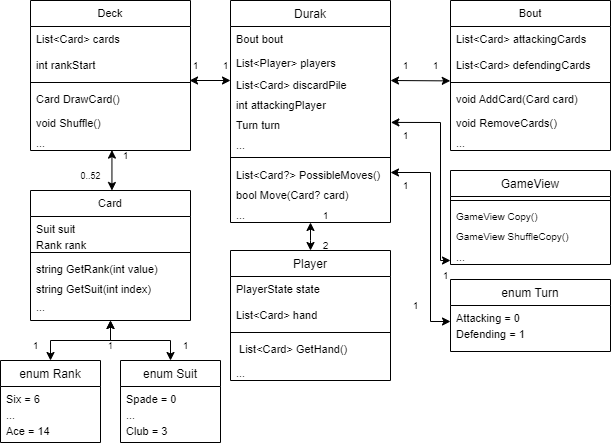
\includegraphics[width=0.9\textwidth]{../img/modelUML.png}
    \caption{A simplified UML diagram showing the relationship between the objects within the Model library.}
    \label{fig:modelUML}
\end{figure}

Before delving into the description of the game state and components of Durak, it is useful to first consider the relationship of all of the objects in the model to that state. A class diagram illustrating the relationships between the objects in the model can be found in Figure \ref{fig:modelUML}.

The representation of the game state \texttt{Durak} in the model is a key aspect of the overall system. This representation holds all of the necessary information and logic required to play the game of Durak, shown in Figure \ref{fig:codeDurak}, and therefore plays a central role in the functioning of the model. As such, it is important to carefully consider the design and implementation of the game state representation along with its components. 

\begin{figure}[h]
\captionsetup{justification=centering}
\lstset{basicstyle=\ttfamily\scriptsize}
\begin{lstlisting}[frame=single]
// Bout object of the game
private Bout bout;

// Deck object of the game
private Deck deck;

// Trump card of the game that can be assigned or not
private Card? trumpCard;

// Representation of the discard pile in the game
private List<Card> discardPile = new List<Card>();

// Players inside the game
private List<Player> players = new List<Player>();

\end{lstlisting}
\caption{A simplified diagram of the Durak class, which encompasses the main properties of the game}
\label{fig:codeDurak}
\end{figure}

The object in question serves as a comprehensive representation of all game states and data throughout a single game of Durak. Because of that it is utilized to communicate this information to other components within the system, such as the command-line interface (CLI) or artificial intelligence (AI) scripts. To facilitate communication and coordination between the Durak model and the agents that interact with it, the game state provides two primary functions: \texttt{PossibleMoves}, shown in Figure \ref{fig:codePossibleMoves} and \texttt{Move}, shown in Figure \ref{fig:codeMove}. These functions serve as the primary means through which changes can be made to the game state, and as such, play a crucial role in the overall operation of the model. 

\begin{figure}[h]
\captionsetup{justification=centering}
\lstset{basicstyle=\ttfamily\scriptsize}
\begin{lstlisting}[frame=single]

if (turn == Turn.Attacking){
	if (CanAttack() && OpponentCanFitMoreCards()) {
		return GenerateListOfAttackingCards();
	} else {
		// passing the attack
		return null;	
	}
}
else {
	Card attackingCard = bout.GetAttackingCards()[^1]
	if (CanDefend(attackingCard)) {
		return GenerateListofDefendingCards(attackingCard);
	} else {
		// taking the cards
		return null
	}
}
\end{lstlisting}
\caption{A simplified overview of the PossibleMoves method inside the Durak class}
\label{fig:codePossibleMoves}
\end{figure}

The \texttt{PossibleMoves} method determines the list of actions that are available to the current player based on the current game state and the rules of the game. When it is the attacker's turn, the method considers the rules for attacking (details in section \ref{attackconditions}) and generates a list of eligible cards that can be played or allows the player to pass if no suitable cards are available. Similarly, when it is the defender's turn (details in section \ref{BeatingRule}), the method takes into account the card being attacked and generates a list of cards that can be played to defend or offers the option to take the attack if no suitable defense is available. This enables the method to adapt to the specific circumstances of the game and provide appropriate options for the current player to make a move.

The \texttt{Move} method modifies the current game state by executing the action chosen by the current player. This move is selected by the agent, which performs calculations based on the possible moves generated by the \texttt{PossibleMoves} method. The specific nature of these calculations depends on the type of agent being used. For example, a rule-based agent may simply select the lowest value rank card, while a more sophisticated agent, such Monte-Carlo Tree Search (MCTS), may use more complex decision-making processes to determine the optimal move to make. Regardless of the type of agent being used, the \texttt{Move} method ultimately updates the game state to reflect the chosen action and advances the game to the next turn.

\begin{figure}[h]
\captionsetup{justification=centering}
\begin{lstlisting}[frame=single]
if (turn == Turn.Attacking){
	// the attacker played a card	
	if (card is not null) {
		attacker.GetHand().Remove(card);
		bout.AddCard(card);
	} else {
		bout.RemoveCards();
		return;
	}
}
else {
	// the defender beat the attacking card
	if (card is not null){
		defender.GetHand().Remove(card);
		bout.AddCard(card);
	} else {
		FillPlayerHand(bout.GetEverything(), defender)
		return;
	}	
}
turn = turn == Turn.Attacking ? Turn.Defending : Turn.Attacking;
\end{lstlisting}
\caption{A simplified overview of the Move method inside the Durak class}
\label{fig:codeMove}
\end{figure}

Additionally, it is important to note that, for security purposes, the agents are not provided with the entire \texttt{Durak} object. Instead, they are given access to a \texttt{GameView} class representation, which allows them to obtain essential information about the current game state and make changes through the methods outlined in Figures \ref{fig:codePossibleMoves} and \ref{fig:codeMove}. This approach ensures that the agents are not able to manipulate the game in an unauthorized manner.


\subsection{CLI}
\label{CLI}

The command-line interface (CLI) plays a crucial role in the architecture of the application. Through the CLI, the user can interact with the application using a text-based interface, providing parameters and receiving feedback or results. The CLI enables a range of experimental and testing scenarios, including the ability to conduct playouts between different agents within a customizable game environment that can be modified by altering various parameters. The flexibility and versatility of the CLI is crucial for exploring the capabilities of the system and evaluating the performance of the AI agents. In this chapter, we will examine the various parameters that can be used to manipulate the behavior of the agents and the game environment through the CLI. This will provide insight into the capabilities of the system and enable a more thorough evaluation of the AI agents' performance.

Before discussing the organizational structure of the project, it is important to introduce the parameters and their roles within the project (Please refer to Figure \ref{fig:parameters}). This will facilitate a better understanding of the various components and how they interact with one another. 

\begin{figure}[h]
\captionsetup{justification=centering}
\begin{lstlisting}[frame=single]
/ai1            : The agent for player 1. (String)(Default = random)
/ai2            : The agent for player 2. (String)(Default = random)
/config         : Used for grid search parameter configuration.(Default = False)
/d1             : Displays # of states & depth for minimax move(Default = False)
/d2             : Displays all the moves that minimax considers(Default = False)
/include_trumps : Enable trump cards in the game(Default = True)
/log            : Enable logs for writing in the file(Default = False)
/open_world     : Make all cards visible to both players(Default = False)
/seed           : A seed for random number generation(Int32)
/start_rank     : The starting rank of cards in the deck(Int32)(Default = 6)
/total_games    : The number of games to play(Int32)(Default = 1000)
/tournament     : Runs the tournament with the agents specified.
/verbose        : Enable verbose output(Default = False)

\end{lstlisting}
\caption{A text-based 'Help' statement that describes the parameters that can be used}
\label{fig:parameters}
\end{figure}

There are various ways to utilize the aforementioned parameters. An example of using the default settings to run a game between RandomAI agent and GreedyAI agent is provided below:

\begin{lstlisting}[frame=single]
dotnet run --project CLI -ai1=random -ai2=greedy
\end{lstlisting}

This command initiates the simulation of 1000 games between the RandomAI and GreedyAI agents in a fully enclosed environment (with a starting rank of 6) and provides the following output to the console:

\begin{lstlisting}[frame=single]
==== RUNNING ====

Game 1: Agent 1 (random) won. Total bouts: 21
Game 2: Agent 2 (greedy) won. Total bouts: 19
Game 3: Agent 2 (greedy) won. Total bouts: 13
Game 4: Agent 2 (greedy) won. Total bouts: 18
Game 5: Agent 2 (greedy) won. Total bouts: 18
...
\end{lstlisting}

To more thoroughly analyze the results of the specific game, \texttt{seed} with the game id and the \texttt{-verbose}  parameters may be utilized. This provides detailed information about the progression of the game by showing every possible move, the chosen move and other game related details. An example of the first game in which a RandomAI agent defeats a GreedyAI agent using this parameter is shown below:


\begin{lstlisting}[frame=single]
dotnet run --project CLI -ai1=random -ai2=greedy -verbose -seed=1
\end{lstlisting}

The command above generates a verbose output, as shown below. It should be noted that this is only a portion of the full output and the blue colored suits are the indications of the trump suit.

\begin{lstlisting}[frame=single]
==== START ====

Trump card: A(*@$\textcolor{blue}{\diamondsuit}$@*)
Deck's size: 36

Player 1 (random) cards: 9(*@$\textcolor{black}{\spadesuit}$@*)  A(*@$\textcolor{black}{\spadesuit}$ @*) 10(*@$\textcolor{red}{\heartsuit}$@*)  Q(*@$\textcolor{red}{\heartsuit}$@*)  9(*@$\textcolor{blue}{\diamondsuit}$@*)  K(*@$\textcolor{blue}{\diamondsuit}$@*)
Player 2 (greedy) cards: 6(*@$\textcolor{black}{\spadesuit}$@*)  8(*@$\textcolor{black}{\spadesuit}$@*)  Q(*@$\textcolor{black}{\spadesuit}$@*)  7(*@$\textcolor{red}{\heartsuit}$@*)  A(*@$\textcolor{red}{\heartsuit}$@*)  6(*@$\textcolor{black}{\clubsuit}$@*)

=== New Bout ===

TURN: Player 1 (random) (Attacking)
Can attack
Possible cards: 9(*@$\textcolor{black}{\spadesuit}$@*)  A(*@$\textcolor{black}{\spadesuit}$@*)  10(*@$\textcolor{red}{\heartsuit}$@*)  Q(*@$\textcolor{red}{\heartsuit}$@*)  9(*@$\textcolor{blue}{\diamondsuit}$@*)  K(*@$\textcolor{blue}{\diamondsuit}$@*)
Attacks: 9(*@$\textcolor{black}{\spadesuit}$@*)

Bout 1:
Attacking cards: 9(*@$\textcolor{black}{\spadesuit}$@*)
Defending cards:

TURN: Player 2 (greedy) (Defending)
Can defend
Possible cards: Q(*@$\textcolor{black}{\spadesuit}$@*)
Defends: Q(*@$\textcolor{black}{\spadesuit}$@*)

Bout 1:
Attacking cards: 9(*@$\textcolor{black}{\spadesuit}$@*)
Defending cards: Q(*@$\textcolor{black}{\spadesuit}$@*)
...
\end{lstlisting}

It is important to consider that when utilizing certain advanced agents, such as Monte-Carlo Tree Search (MCTS) and Minimax, it is necessary to specify their respective parameters in order to effectively utilize their capabilities. 

In the context of the Minimax algorithm, it is necessary to specify the value of the \texttt{depth} parameter, which determines the depth to which the search tree will be explored in order to identify the optimal move. In addition to the depth parameter, it is also necessary to specify the \texttt{eval} parameter, which specifies the heuristic function used to evaluate the state when the maximum depth has been reached. The \texttt{eval} parameter can take on either the value "basic" or "playout" (additional information on these parameters can be found in Section \ref{minimax}). It is worth noting that, in a closed world scenario, the \texttt{samples} parameter is optional and has a default value of 20. The \texttt{samples} parameter serves to prevent agents such as Minimax and MCTS from cheating by accessing information about future states of the game (details in Section \ref{AIAgents}). This illustration presents an example of a simulation between the Minimax and greedy agents with arbitrary parameter values in the open and closed world:\\

\textbf{Open-world: }
\begin{lstlisting}[frame=single]
dotnet run --project CLI -ai1=minimax:depth=4,eval=basic -ai2=greedy -open_world
\end{lstlisting}

\textbf{Closed-world: }
\begin{lstlisting}[frame=single]
dotnet run --project CLI -ai1=minimax:depth=6,eval=basic,samples=15 -ai2=smart
\end{lstlisting}

Regarding MCTS, it is necessary to specify the value of the \texttt{limit} parameter, which determines the computational budget allocated for the algorithm to build the search tree. The search is halted and the best-performing root action is returned once this budget is reached. The \texttt{c}, which is called exploration constant, parameter also needs to be specified because it determines the balance between exploitation and exploration in the UCB equation(detailed information is provided in Section \ref{MCTS}). This parameter is set to a default value of  $\sqrt{2}$ ($\approx 1.41$) and can be adjusted to fine-tune the performance of the algorithm. The \texttt{simulation} parameter should also be specified, indicating whether to use a smart simulation ("greedy") or a random simulation ("random"). Lastly, in a closed world setting, just like in Minimax, it is necessary to specify the \texttt{samples} parameter to prevent the MCTS agent from cheating by considering future states of the game. This example demonstrates a simulation between MCTS and greedy agents with arbitrary parameter values in open and closed world settings: \\

\textbf{Open-world: }
\begin{lstlisting}[frame=single]
dotnet run --project CLI -ai1=mcts:limit=100,simulation=greedy -ai2=greedy 
							-open_world
\end{lstlisting}

\textbf{Closed-world: }
\begin{lstlisting}[frame=single]
dotnet run --project CLI -ai1=mcts:limit=100,simulation=greedy,samples=10 
							-ai2=greedy
\end{lstlisting}



\subsection{AI Agents}

